\documentclass{beamer}
\usepackage[utf8]{inputenc}
\usepackage{graphicx}
\usetheme{Warsaw}
\usecolortheme{seahorse}

\title{Cancer Analysis Workflow Sprint Review}
%\author{P. Akan, J. Eisfeldt, M. Garcia, S. Juhos, M. Käller, M. Larsson, B. Nystedt, P. Olason}
\institute{SciLifeLab}
\date{18th Aug. 2016 }
\begin{document}
\frame{\titlepage}
			  
\begin{frame}
\frametitle{Cancer Analysis Workflow Sprint Review}
\begin{itemize}
	\item Which parts are ready so far?
	\item Things waiting to be completed
	\item Abandoned parts
	\item Yet to come
\end{itemize}
\end{frame}

\begin{frame}
\frametitle{Where Are We Now?}
\begin{block}{We had bubbles}
Sub-sets for each step as pre-processing, variant call, structural variants, annotation ...
\end{block}
\center{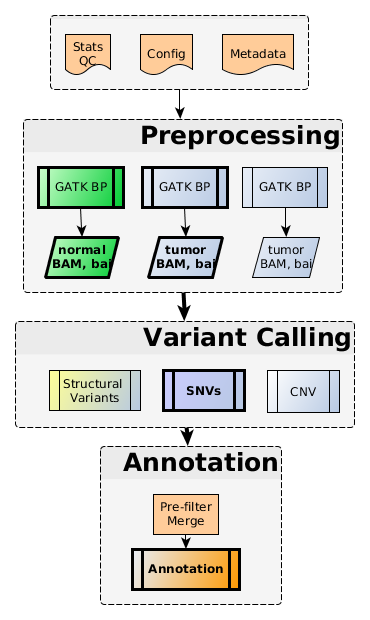
\includegraphics[width=0.34\linewidth]{General_schema.png}}
\end{frame}

\begin{frame}
\frametitle{Where Are We Now?}
\begin{block}{Now we have}
	Actual directories containing data, variant calls and alignment files

	Still in the benchmarking phase
\end{block}
\begin{block}{First benchmarking: TCGA DREAM challenge}
	\begin{itemize}
		\item Three phases, gradually more difficult to do variant call
		\item Set of tumour/normal contamination ratios
		\item ''Gold standard'' of somatic variant calls
		\item It is still a simulated somatic mutation set, not real data
	\end{itemize}
\end{block}
There are other real data cases to benchmark against, but first we are have to go through these steps
\end{frame}


\begin{frame}
\frametitle{Where Are We Now?}
\begin{block}{Hardware requirements}
	\begin{itemize}
		\item Goal is to have a workflow that can be used on UPPMAX clusters
		\item In fact on any Linux system
		\item Nextflow makes it possible to deploy easily anywhere, but additional software (bwa/GATK/etc) have to be installed
	\end{itemize}
\end{block}
\begin{block}{Installing}
	\begin{itemize}
		\item it took $\sim$2 days to set up everything from scratch
		\item on UPPMAX the actual configuration should should work - to be honest you need some tweaking on irma
		\item Setting up things on a cluster from scratch: tried on a simple emulated case, it is more or less the same as on a single big machine
		\item \alert{Storage is and will be an issue more than CPU time}
	\end{itemize}
\end{block}
\end{frame}

\begin{frame}
\frametitle{Software Implementation Details}
\begin{block}{Keeping an eye on Broad's workflow}
	\begin{itemize}
		\item Preprocessing: GATK best practices - originally only the WGS practices were followed, but our schema is pretty like the recent GATK somatic flow
		\item Not only tumour/normal, but relapse or additional stages are included
	\end{itemize}
\end{block}
\begin{block}{Spread and gather:}
	\begin{itemize}
		\item For variant callers we chop up the chromosomes at centromers and feed the fragments each on a separate machine instead of running the whole thing on a single one 
		\item Still, VarDictJava eats up all the memory
	\end{itemize}
\end{block}
\end{frame}

\begin{frame}
\frametitle{Variant Calling - 35 somatic callers on this list}
\center{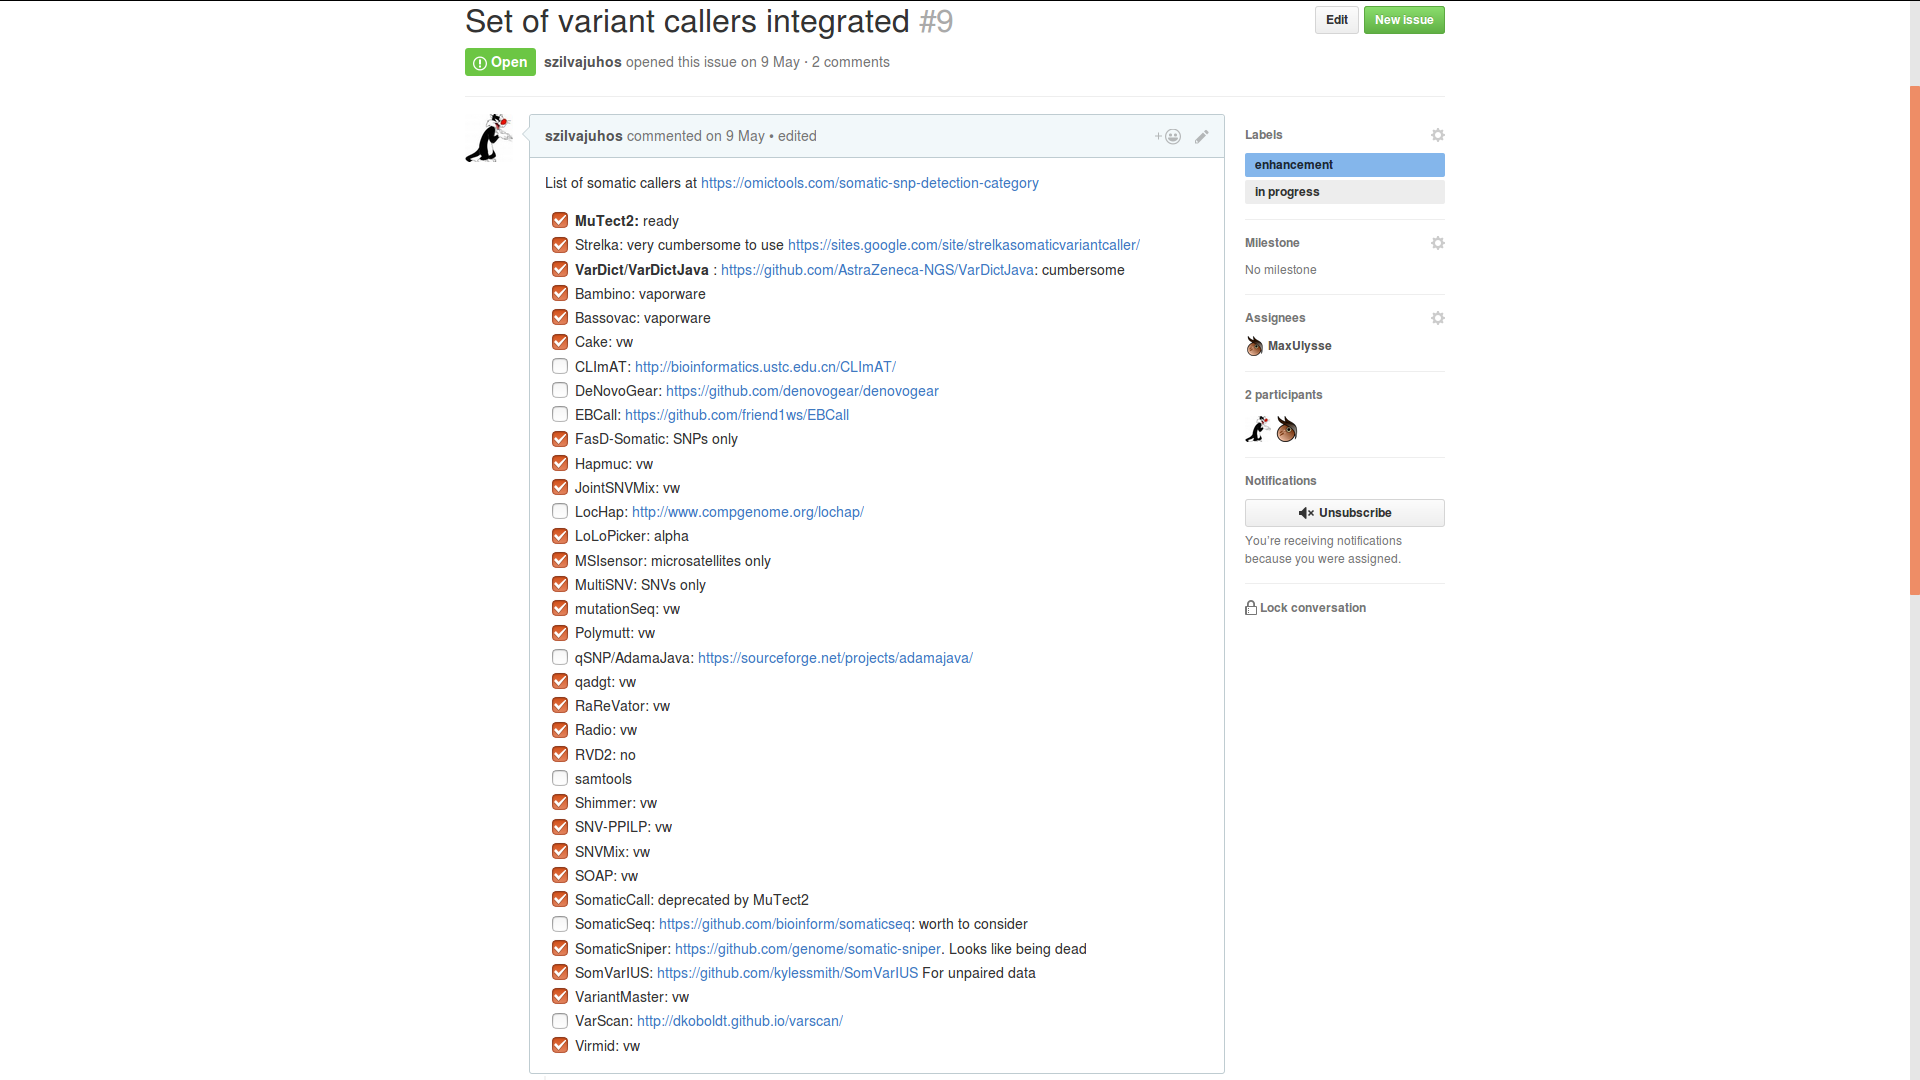
\includegraphics[width=1.2\linewidth]{VCs_integrated.png}}
\end{frame}

\begin{frame}
\frametitle{Variant Calling}
\begin{block}{We love MuTect2}
	\begin{itemize}
		\item we love it, because it at least works
		\item and is not eating up the machine
		\item and uses standard files
	\end{itemize}
\end{block}
\begin{block}{We have an ambivalent relationship towards VarDict and Strelka}
	\begin{itemize}
		\item VarDict is pretty cumbersome to use, and memory-hungry
		\item For Strelka you have to have specially prepared files
	\end{itemize}
\end{block}
\end{frame}

\begin{frame}
\frametitle{VarDict In Action}
\center{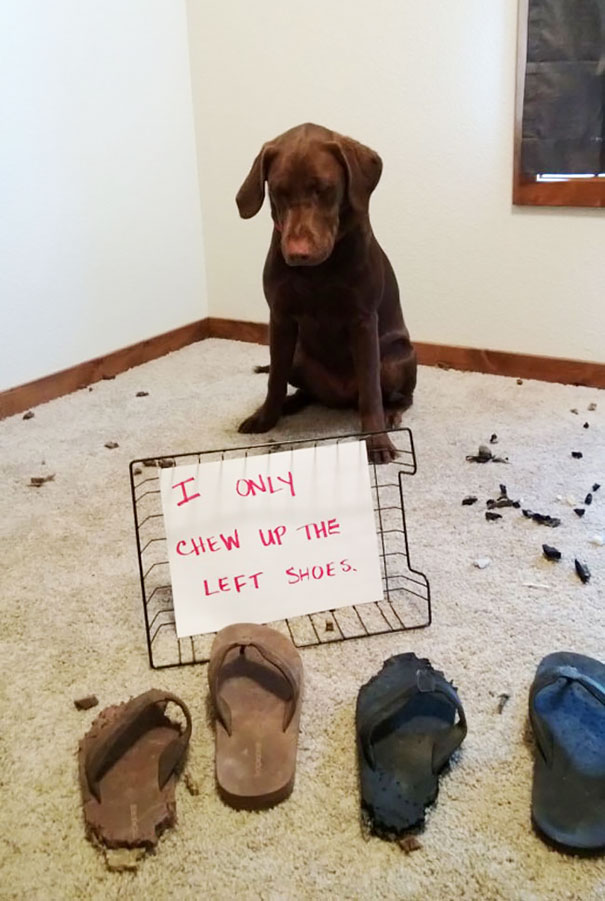
\includegraphics[width=0.5\linewidth]{dogEating.jpg}}
\end{frame}

\begin{frame}
\frametitle{Structural Variants}
\begin{itemize}
	\item Original plan was not to include them at all
	\item Mostly Jesper's part
	\item It must be there for cancer
\end{itemize}
\begin{block}{Issues:}
\begin{itemize}
	\item Difficult to find validation data
	\item Needs IT resources (disk/CPU) even for a simple validation
\end{itemize}
We are in a special position as 10X sequencing can be used for cross-validation

It will be still resource-hungry
\end{block}
\end{frame}

\begin{frame}
\frametitle{Structural Variants}
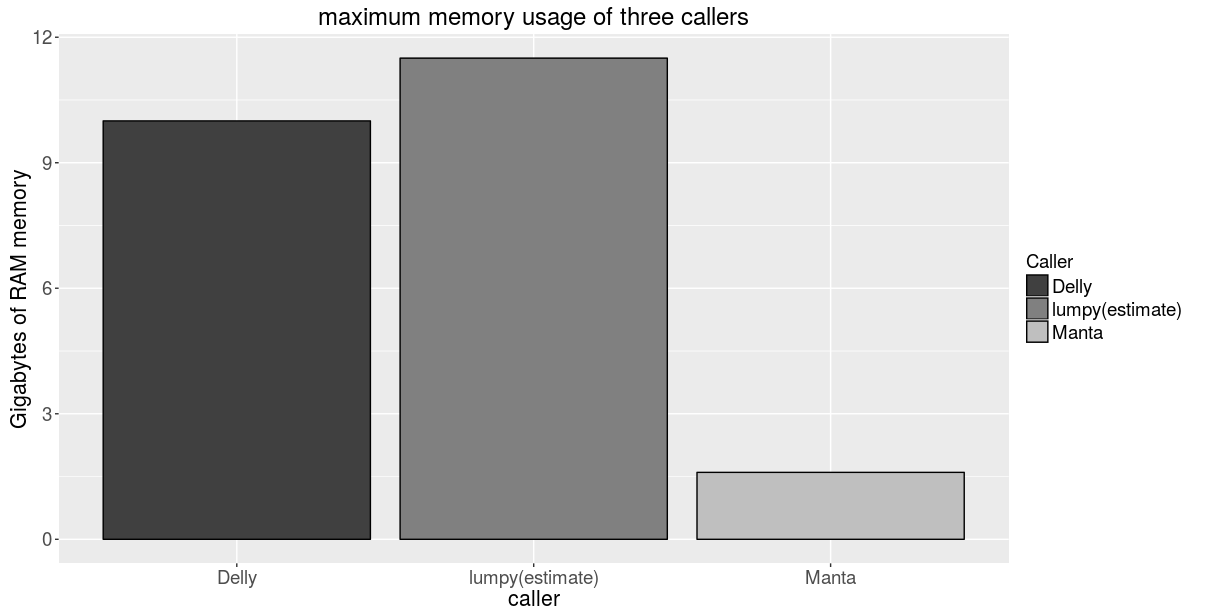
\includegraphics[width=1.0\linewidth]{memory_usage.png}
\end{frame}

\begin{frame}
\frametitle{Structural Variants}
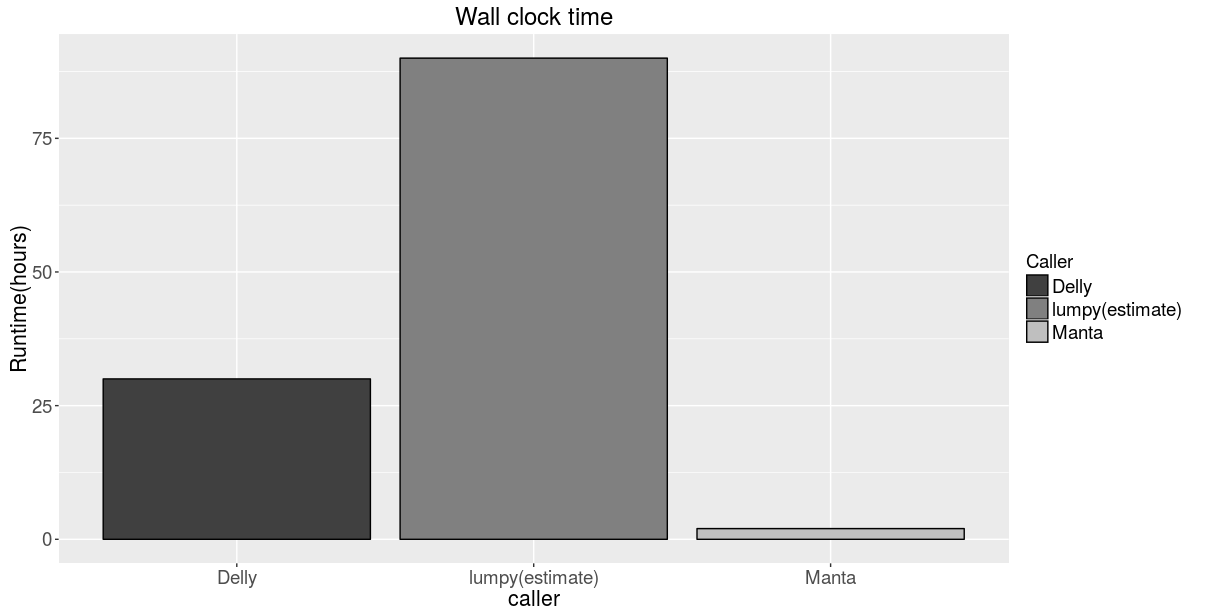
\includegraphics[width=1.0\linewidth]{wall_clock.png}
\end{frame}

\begin{frame}
\frametitle{Structural Variants}
	\begin{block}{Software tested}
	Goal was to benchmark first the available options
	\end{block}
	\begin{itemize}		
		\item Lumpy: crashed after 48 hours of runtime 
		\item Delly: you can switch off some of its modules, but you will not get all the SVs
		\item Manta: fast, precise and sensitive
	\end{itemize}
	\begin{block}{For now there is only one SV caller to be added}
	They have similar sensitivity for most variant types, but in general manta has higher precision

	As Manta is the one that performs best in the tests and fast enough, it is in the workflow
	\end{block}
\end{frame}

\begin{frame}
\frametitle{Structural Variants - 10X Chromium}
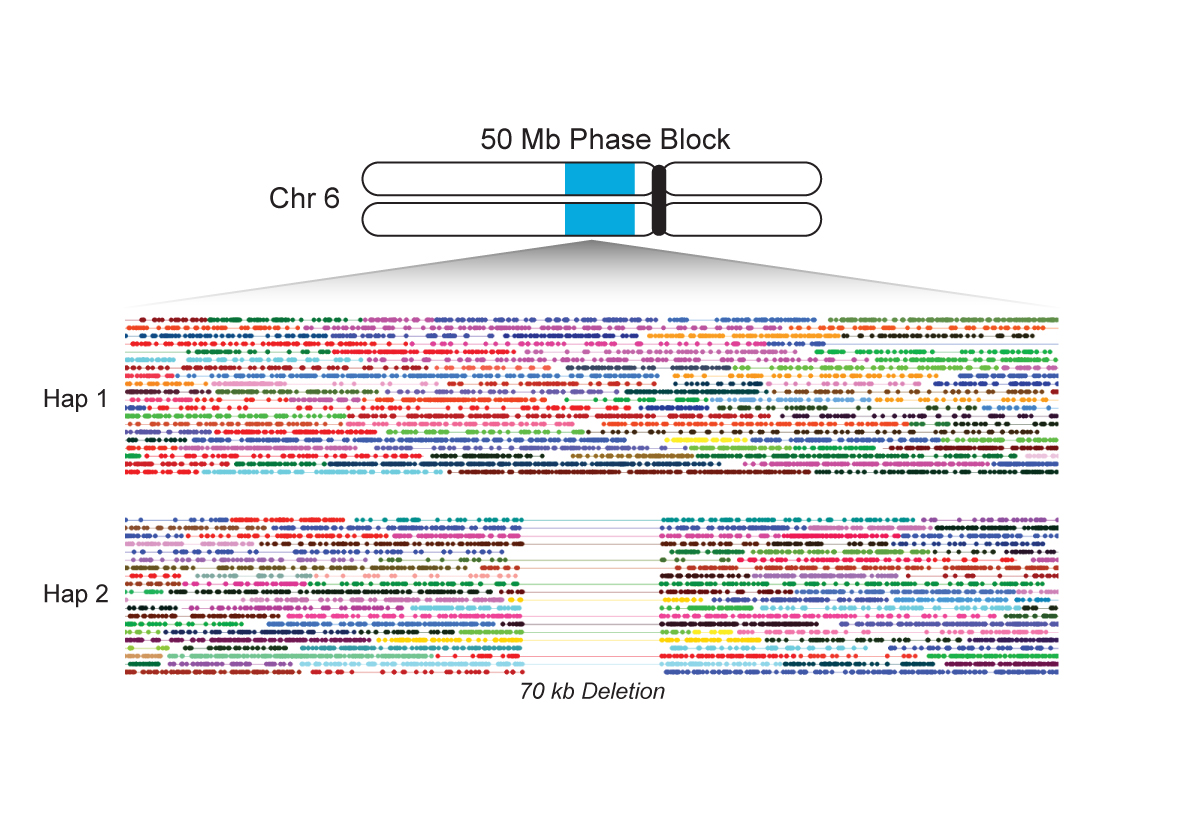
\includegraphics[width=1.0\linewidth]{multi-megabase-phase-blocks-large.jpg}
\end{frame}

\begin{frame}
\frametitle{Structural Variants}
\includegraphics[width=1.0\linewidth]{10x_chromium_1st_run.png}
\end{frame}

\begin{frame}
\frametitle{Purity, ploidy and CNVs}
\begin{block}{ASCAT}
	It is working separately, but not integrated into the workflow yet.

	Gave a hard time to make it work in first place: it is not designed for NGS data.
	
	Adds important numbers about:
	\begin{itemize}
		\item tumour purity
		\item average ploidy
		\item ploidy for individual chromosomes
		\item allele-specific copy numbers
	\end{itemize}
\end{block}
\end{frame}

\begin{frame}
\frametitle{Cancer Analysis Workflow Sprint Review}
\begin{itemize}
	\item Which parts are ready so far?
		\begin{itemize}
			\item Preprocessing
			\item Normal / Tumour / Relapse steps
			\item Dealing with read groups
			\item MuTect2 (and VarDict if you have enough memory)
		\end{itemize}
	\item Things waiting to be completed
		\begin{itemize}
			\item Strelka - and maybe yet an other variant caller
			\item ASCAT
			\item Manta (ready but not tested thoroughly)
			\item merging results
		\end{itemize}
	\item Abandoned parts
		\begin{itemize}
			\item Many potential variant callers
		\end{itemize}
	\item Yet to come
		\begin{itemize}
			\item Annotation (prototype is ready)
			\item Visualization
			\item Data mining / AI / SVM to eliminate false positives
		\end{itemize}
\end{itemize}
\end{frame}

\begin{frame}
\frametitle{The Alphabetical List}
\begin{itemize}
	\item Jesper Eisfeldt
	\item Maxime Garcia 
	\item Szilveszter Juhos 
	\item Max Käller
	\item Malin Larsson
	\item Björn Nystedt 
	\item Pall Olason
	\item Pelin Sahlen
	\item Teresita Díaz De Ståhl
\end{itemize}
\end{frame}

\begin{frame}
\frametitle{Short-term TODO}
	\begin{itemize}
		\item Make the GitHub repository public, so everybody can follow what is going on
		\item Survey storage usage: storage is already an issue, likely we have to implement something that cleans up previous steps
		\item Germline variants: these are already shipped in the standard NGI pipeline, and it should be "trivial" to add
		\item MuTect2 in DREAM challenge: have to look up how it performs
		\item Strelka and MuTect1 as default variant callers
	\end{itemize} 
\end{frame}


\begin{frame}
\frametitle{Longer-term TODO}
	\begin{itemize}
		\item Benchmark Manta
		\item Malin is going to give a long presentation about ASCAT and related software on Tue, 13th Sept 13:00 in Alpha 3 Big (room booked)
		\item Add ASCAT as a module to the workflow
		\item Merge variant calls from different callers into a singe result file
		\item Go through all the TCGA DREAM challenge benchmarking steps S1, S2, S3
		\item We are expecting that for the next review we have benchmark data and some real data processed
		\item Next meeting in Thu, 13th Oct. 10:00 Alpha 3 Big (room booked)
	\end{itemize}
\end{frame}

\end{document}
